% Options for packages loaded elsewhere
% Options for packages loaded elsewhere
\PassOptionsToPackage{unicode}{hyperref}
\PassOptionsToPackage{hyphens}{url}
%
\documentclass[
  english,
  russian,
  12pt,
  a4paper,
  DIV=11,
  numbers=noendperiod]{scrreprt}
\usepackage{xcolor}
\usepackage[top=30mm,left=20mm,right=20mm,bottom=30mm]{geometry}
\usepackage{amsmath,amssymb}
\setcounter{secnumdepth}{5}
\usepackage{iftex}
\ifPDFTeX
  \usepackage[T1]{fontenc}
  \usepackage[utf8]{inputenc}
  \usepackage{textcomp} % provide euro and other symbols
\else % if luatex or xetex
  \usepackage{unicode-math} % this also loads fontspec
  \defaultfontfeatures{Scale=MatchLowercase}
  \defaultfontfeatures[\rmfamily]{Ligatures=TeX,Scale=1}
\fi
\usepackage{lmodern}
\ifPDFTeX\else
  % xetex/luatex font selection
  \setmainfont[]{DejaVu Serif}
  \setmonofont[]{DejaVu Sans Mono}
\fi
% Use upquote if available, for straight quotes in verbatim environments
\IfFileExists{upquote.sty}{\usepackage{upquote}}{}
\IfFileExists{microtype.sty}{% use microtype if available
  \usepackage[]{microtype}
  \UseMicrotypeSet[protrusion]{basicmath} % disable protrusion for tt fonts
}{}
\usepackage{setspace}
% Make \paragraph and \subparagraph free-standing
\makeatletter
\ifx\paragraph\undefined\else
  \let\oldparagraph\paragraph
  \renewcommand{\paragraph}{
    \@ifstar
      \xxxParagraphStar
      \xxxParagraphNoStar
  }
  \newcommand{\xxxParagraphStar}[1]{\oldparagraph*{#1}\mbox{}}
  \newcommand{\xxxParagraphNoStar}[1]{\oldparagraph{#1}\mbox{}}
\fi
\ifx\subparagraph\undefined\else
  \let\oldsubparagraph\subparagraph
  \renewcommand{\subparagraph}{
    \@ifstar
      \xxxSubParagraphStar
      \xxxSubParagraphNoStar
  }
  \newcommand{\xxxSubParagraphStar}[1]{\oldsubparagraph*{#1}\mbox{}}
  \newcommand{\xxxSubParagraphNoStar}[1]{\oldsubparagraph{#1}\mbox{}}
\fi
\makeatother

\usepackage{color}
\usepackage{fancyvrb}
\newcommand{\VerbBar}{|}
\newcommand{\VERB}{\Verb[commandchars=\\\{\}]}
\DefineVerbatimEnvironment{Highlighting}{Verbatim}{commandchars=\\\{\}}
% Add ',fontsize=\small' for more characters per line
\usepackage{framed}
\definecolor{shadecolor}{RGB}{248,248,248}
\newenvironment{Shaded}{\begin{snugshade}}{\end{snugshade}}
\newcommand{\AlertTok}[1]{\textcolor[rgb]{0.94,0.16,0.16}{#1}}
\newcommand{\AnnotationTok}[1]{\textcolor[rgb]{0.56,0.35,0.01}{\textbf{\textit{#1}}}}
\newcommand{\AttributeTok}[1]{\textcolor[rgb]{0.13,0.29,0.53}{#1}}
\newcommand{\BaseNTok}[1]{\textcolor[rgb]{0.00,0.00,0.81}{#1}}
\newcommand{\BuiltInTok}[1]{#1}
\newcommand{\CharTok}[1]{\textcolor[rgb]{0.31,0.60,0.02}{#1}}
\newcommand{\CommentTok}[1]{\textcolor[rgb]{0.56,0.35,0.01}{\textit{#1}}}
\newcommand{\CommentVarTok}[1]{\textcolor[rgb]{0.56,0.35,0.01}{\textbf{\textit{#1}}}}
\newcommand{\ConstantTok}[1]{\textcolor[rgb]{0.56,0.35,0.01}{#1}}
\newcommand{\ControlFlowTok}[1]{\textcolor[rgb]{0.13,0.29,0.53}{\textbf{#1}}}
\newcommand{\DataTypeTok}[1]{\textcolor[rgb]{0.13,0.29,0.53}{#1}}
\newcommand{\DecValTok}[1]{\textcolor[rgb]{0.00,0.00,0.81}{#1}}
\newcommand{\DocumentationTok}[1]{\textcolor[rgb]{0.56,0.35,0.01}{\textbf{\textit{#1}}}}
\newcommand{\ErrorTok}[1]{\textcolor[rgb]{0.64,0.00,0.00}{\textbf{#1}}}
\newcommand{\ExtensionTok}[1]{#1}
\newcommand{\FloatTok}[1]{\textcolor[rgb]{0.00,0.00,0.81}{#1}}
\newcommand{\FunctionTok}[1]{\textcolor[rgb]{0.13,0.29,0.53}{\textbf{#1}}}
\newcommand{\ImportTok}[1]{#1}
\newcommand{\InformationTok}[1]{\textcolor[rgb]{0.56,0.35,0.01}{\textbf{\textit{#1}}}}
\newcommand{\KeywordTok}[1]{\textcolor[rgb]{0.13,0.29,0.53}{\textbf{#1}}}
\newcommand{\NormalTok}[1]{#1}
\newcommand{\OperatorTok}[1]{\textcolor[rgb]{0.81,0.36,0.00}{\textbf{#1}}}
\newcommand{\OtherTok}[1]{\textcolor[rgb]{0.56,0.35,0.01}{#1}}
\newcommand{\PreprocessorTok}[1]{\textcolor[rgb]{0.56,0.35,0.01}{\textit{#1}}}
\newcommand{\RegionMarkerTok}[1]{#1}
\newcommand{\SpecialCharTok}[1]{\textcolor[rgb]{0.81,0.36,0.00}{\textbf{#1}}}
\newcommand{\SpecialStringTok}[1]{\textcolor[rgb]{0.31,0.60,0.02}{#1}}
\newcommand{\StringTok}[1]{\textcolor[rgb]{0.31,0.60,0.02}{#1}}
\newcommand{\VariableTok}[1]{\textcolor[rgb]{0.00,0.00,0.00}{#1}}
\newcommand{\VerbatimStringTok}[1]{\textcolor[rgb]{0.31,0.60,0.02}{#1}}
\newcommand{\WarningTok}[1]{\textcolor[rgb]{0.56,0.35,0.01}{\textbf{\textit{#1}}}}

\usepackage{longtable,booktabs,array}
\usepackage{calc} % for calculating minipage widths
% Correct order of tables after \paragraph or \subparagraph
\usepackage{etoolbox}
\makeatletter
\patchcmd\longtable{\par}{\if@noskipsec\mbox{}\fi\par}{}{}
\makeatother
% Allow footnotes in longtable head/foot
\IfFileExists{footnotehyper.sty}{\usepackage{footnotehyper}}{\usepackage{footnote}}
\makesavenoteenv{longtable}
\usepackage{graphicx}
\makeatletter
\newsavebox\pandoc@box
\newcommand*\pandocbounded[1]{% scales image to fit in text height/width
  \sbox\pandoc@box{#1}%
  \Gscale@div\@tempa{\textheight}{\dimexpr\ht\pandoc@box+\dp\pandoc@box\relax}%
  \Gscale@div\@tempb{\linewidth}{\wd\pandoc@box}%
  \ifdim\@tempb\p@<\@tempa\p@\let\@tempa\@tempb\fi% select the smaller of both
  \ifdim\@tempa\p@<\p@\scalebox{\@tempa}{\usebox\pandoc@box}%
  \else\usebox{\pandoc@box}%
  \fi%
}
% Set default figure placement to htbp
\def\fps@figure{htbp}
\makeatother



\ifLuaTeX
\usepackage[bidi=basic,provide=*]{babel}
\else
\usepackage[bidi=default,provide=*]{babel}
\fi
\ifPDFTeX
\else
\babelfont{rm}[]{DejaVu Serif}
\fi
% get rid of language-specific shorthands (see #6817):
\let\LanguageShortHands\languageshorthands
\def\languageshorthands#1{}


\setlength{\emergencystretch}{3em} % prevent overfull lines

\providecommand{\tightlist}{%
  \setlength{\itemsep}{0pt}\setlength{\parskip}{0pt}}



 
\usepackage[style=gost-numeric,backend=biber,langhook=extras,autolang=other*]{biblatex}
\addbibresource{bib/cite.bib}

\usepackage[]{csquotes}

\usepackage{indentfirst}
\usepackage{float}
\usepackage{juliamono}
\floatplacement{figure}{H}
\IfFileExists{plex-otf.sty}{
  %% Full TeXlive
  \usepackage[
    % math,
    RM={Scale=0.94},SS={Scale=0.94},SScon={Scale=0.94},TT={Scale=MatchLowercase,FakeStretch=0.9},
    DefaultFeatures={Ligatures=Common}
  ]{plex-otf}
  % \usepackage[Scale=MatchUppercase]{juliamono}
}{
  %% TinyTeX
  \usepackage{libertine}
}
\KOMAoption{captions}{tableheading}
\makeatletter
\@ifpackageloaded{caption}{}{\usepackage{caption}}
\AtBeginDocument{%
\ifdefined\contentsname
  \renewcommand*\contentsname{Содержание}
\else
  \newcommand\contentsname{Содержание}
\fi
\ifdefined\listfigurename
  \renewcommand*\listfigurename{Список иллюстраций}
\else
  \newcommand\listfigurename{Список иллюстраций}
\fi
\ifdefined\listtablename
  \renewcommand*\listtablename{Список таблиц}
\else
  \newcommand\listtablename{Список таблиц}
\fi
\ifdefined\figurename
  \renewcommand*\figurename{Рисунок}
\else
  \newcommand\figurename{Рисунок}
\fi
\ifdefined\tablename
  \renewcommand*\tablename{Таблица}
\else
  \newcommand\tablename{Таблица}
\fi
}
\@ifpackageloaded{float}{}{\usepackage{float}}
\floatstyle{ruled}
\@ifundefined{c@chapter}{\newfloat{codelisting}{h}{lop}}{\newfloat{codelisting}{h}{lop}[chapter]}
\floatname{codelisting}{Список}
\newcommand*\listoflistings{\listof{codelisting}{Листинги}}
\makeatother
\makeatletter
\makeatother
\makeatletter
\@ifpackageloaded{caption}{}{\usepackage{caption}}
\@ifpackageloaded{subcaption}{}{\usepackage{subcaption}}
\makeatother
\usepackage{bookmark}
\IfFileExists{xurl.sty}{\usepackage{xurl}}{} % add URL line breaks if available
\urlstyle{same}
\hypersetup{
  pdftitle={Отчёт по лабораторной работе №3},
  pdfauthor={Малюга Валерия Васильевна},
  pdflang={ru},
  hidelinks,
  pdfcreator={LaTeX via pandoc}}


\title{Отчёт по лабораторной работе №3}
\usepackage{etoolbox}
\makeatletter
\providecommand{\subtitle}[1]{% add subtitle to \maketitle
  \apptocmd{\@title}{\par {\large #1 \par}}{}{}
}
\makeatother
\subtitle{Агентное моделирование}
\author{Малюга Валерия Васильевна}
\date{}
\begin{document}
\maketitle

\renewcommand*\contentsname{Содержание}
{
\setcounter{tocdepth}{1}
\tableofcontents
}
\listoffigures
\listoftables

\setstretch{1.5}
engine: julia

\chapter{Цель
работы}\label{ux446ux435ux43bux44c-ux440ux430ux431ux43eux442ux44b}

Познакомиться с понятием агентного моделирования, создать необходимые
файлы.

\chapter{Задание}\label{ux437ux430ux434ux430ux43dux438ux435}

\begin{itemize}
\tightlist
\item
  Создать рабочий каталог для кода.
\item
  Установить необходимые пакеты.
\item
  Выполнить предложенный код.
\item
  Преобразовать код в литературный стиль.
\item
  Сгенерировать из литературного кода:

  \begin{itemize}
  \tightlist
  \item
    чистый код;
  \item
    jupyter notebook;
  \item
    документацию в формате Quarto.
  \end{itemize}
\item
  Выполнить код из jupyter notebook.
\item
  Интегрировать документацию в формате Quarto в отчёт.
\item
  Добавить в код в литературном стиле вычисление для набора параметров.
\item
  Сгенерировать из литературного кода с параметрами:

  \begin{itemize}
  \tightlist
  \item
    чистый код;
  \item
    jupyter notebook;
  \item
    документацию в формате Quarto.
  \end{itemize}
\item
  Выполнить код из jupyter notebook с параметрами.
\item
  Интегрировать документацию с параметрами в формате Quarto в отчёт.
\item
  Результирующие файлы выложить на git.
\end{itemize}

\chapter{Теоретическое
введение}\label{ux442ux435ux43eux440ux435ux442ux438ux447ux435ux441ux43aux43eux435-ux432ux432ux435ux434ux435ux43dux438ux435}

\section{Агентное
моделирование}\label{ux430ux433ux435ux43dux442ux43dux43eux435-ux43cux43eux434ux435ux43bux438ux440ux43eux432ux430ux43dux438ux435}

Агентный подход (Agent-Based Modeling, ABM) --- это метод исследования
сложных систем, в котором поведение системы возникает из взаимодействия
множества автономных сущностей (агентов). Вместо глобальных уравнений мы
моделируем каждого агента и его правила, а затем наблюдаем коллективные
паттерны \autocite{datseris2022agents}.

\subsection{Основные компоненты агентной
модели}\label{ux43eux441ux43dux43eux432ux43dux44bux435-ux43aux43eux43cux43fux43eux43dux435ux43dux442ux44b-ux430ux433ux435ux43dux442ux43dux43eux439-ux43cux43eux434ux435ux43bux438}

Любая агентная модель включает три основных элемента:

Агенты --- это активные сущности. Они обладают: Свойствами (атрибутами):
возраст, цвет, запас ресурсов, координаты и т.п. Правилами поведения:
как агент реагирует на изменения среды и действия других агентов
(например, перемещение, размножение, потребление). Целями (не
обязательно): в некоторых моделях агенты стремятся максимизировать свою
выгоду или выжить. Способностью к обучению или адаптации (в продвинутых
моделях). Среда --- это пространство, в котором существуют агенты. Она
может быть: Дискретной (клеточная сетка, как в Daisyworld). Непрерывной
(двумерное или трёхмерное пространство). Сетевой (граф социальных
связей). Абстрактной (например, рынок без явных координат). Среда также
может иметь свои свойства (температура, ресурсы) и динамику (диффузия,
обновление).

Взаимодействия --- правила, определяющие, как агенты влияют друг на
друга и на среду. Они могут быть: Локальными (только с соседями).
Глобальными (все агенты взаимодействуют со всеми). Через среду (агенты
изменяют среду, а среда влияет на агентов).

\subsection{Основные
принципы}\label{ux43eux441ux43dux43eux432ux43dux44bux435-ux43fux440ux438ux43dux446ux438ux43fux44b}

Эмерджентность: глобальное поведение системы не закладывается явно, а
возникает из локальных взаимодействий. Это позволяет открывать
неожиданные закономерности. Автономия: агенты действуют независимо, на
основе своей внутренней логики. Гетерогенность: агенты могут различаться
по своим характеристикам и правилам, что отражает реальное разнообразие.
Локальность: чаще всего агенты обладают информацией только о своём
ближайшем окружении.

\section{DaisyWorld}\label{daisyworld}

Модель Daisyworld предложена Джеймсом Лавлоком и Эндрю Уотсоном для
иллюстрации гипотезы Геи \autocite{watson1983,wood2008}. В этом мире на
клеточной сетке растут чёрные и белые маргаритки, различающиеся альбедо
(способностью отражать свет). Чёрные маргаритки поглощают больше тепла,
нагревая среду; белые --- отражают, охлаждая её. Размножение возможно
только в определённом температурном диапазоне. За счёт обратной связи
популяции маргариток стабилизируют планетарную температуру.

\subsection{Описание
модели}\label{ux43eux43fux438ux441ux430ux43dux438ux435-ux43cux43eux434ux435ux43bux438}

В модели Daisyworld агентами являются чёрные и белые маргаритки. Они
живут на клеточной сетке (среда).

Свойства агентов: вид и возраст.

Правила:

Маргаритки изменяют локальную температуру за счёт разного альбедо.
Температура влияет на вероятность размножения (чем ближе к оптимуму, тем
выше шанс заселить соседнюю пустую клетку). Агенты стареют и умирают
после определённого возраста. Среда (температура) диффундирует между
клетками.

\subsection{Агенты и параметры модели
DaisyWorld}\label{ux430ux433ux435ux43dux442ux44b-ux438-ux43fux430ux440ux430ux43cux435ux442ux440ux44b-ux43cux43eux434ux435ux43bux438-daisyworld}

Маргаритки двух типов --- чёрные (black) и белые (white). Каждая
маргаритка занимает одну клетку сетки и имеет возраст (количество шагов
с момента появления). Двумерная квадратная сетка (например, 30×30) с
периодическими границами.

luminosity -- солнечная постоянная (может изменяться со временем).
albedo\_black, albedo\_white -- альбедо чёрных и белых маргариток.
surface\_albedo --- альбедо пустой почвы. max\_age --- максимальный
возраст маргаритки.

\subsection{Динамика}\label{ux434ux438ux43dux430ux43cux438ux43aux430}

Для каждой клетки рассчитывается локальная температура.

Каждая маргаритка может погибнуть с вероятностью, зависящей от
температуры. Если температура выходит за допустимый диапазон,
вероятность смерти повышается.

Если клетка пуста, на неё может попасть семя от соседней маргаритки.
Вероятность успешного прорастания зависит от температуры клетки. Если
вероятность превышает случайное число, на пустой клетке появляется новая
маргаритка того же цвета, что и родительская.

\chapter{Выполнение лабораторной
работы}\label{ux432ux44bux43fux43eux43bux43dux435ux43dux438ux435-ux43bux430ux431ux43eux440ux430ux442ux43eux440ux43dux43eux439-ux440ux430ux431ux43eux442ux44b}

\section{Создание структуры каталогов и установка
пакетов}\label{ux441ux43eux437ux434ux430ux43dux438ux435-ux441ux442ux440ux443ux43aux442ux443ux440ux44b-ux43aux430ux442ux430ux43bux43eux433ux43eux432-ux438-ux443ux441ux442ux430ux43dux43eux432ux43aux430-ux43fux430ux43aux435ux442ux43eux432}

Был создан рабочий каталог и общий проект \texttt{labs/project}
(рис.~\ref{fig-001}). В проект установлены необходимые пакеты:
\texttt{Agents}, \texttt{CairoMakie} и др. (рис. Рисунок~\ref{fig-002}).

\begin{figure}

\centering{


\includegraphics[width=0.7\linewidth,height=\textheight,keepaspectratio]{image/1.png}

}

\caption{\label{fig-001}Структура каталогов лабораторной работы}

\end{figure}%

\begin{figure}

\centering{


\includegraphics[width=0.7\linewidth,height=\textheight,keepaspectratio]{image/2.png}

}

\caption{\label{fig-002}Установленные пакеты в проекте}

\end{figure}%

\section{Реализация
модели}\label{ux440ux435ux430ux43bux438ux437ux430ux446ux438ux44f-ux43cux43eux434ux435ux43bux438}

Файл \texttt{src/daisyworld.jl} содержит определение агента
\texttt{Daisy} и основные функции: обновление температуры, диффузию,
размножение, старение и изменение солнечной активности. Литературная
версия этого файла была оформлена с подробными комментариями.

\section{Базовая
визуализация}\label{ux431ux430ux437ux43eux432ux430ux44f-ux432ux438ux437ux443ux430ux43bux438ux437ux430ux446ux438ux44f}

Скрипт \texttt{scripts/daisyworld\_lit.jl} создаёт модель и сохраняет
три кадра: начальное состояние, после 5 шагов и после 40 шагов (рис.
Рисунок~\ref{fig-basic}). На тепловой карте отображается температура, а
маргаритки показаны символами (чёрные и белые).

\begin{figure}

\centering{


\includegraphics[width=0.7\linewidth,height=\textheight,keepaspectratio]{image/3.png}

}

\caption{\label{fig-basic}Базовая визуализация: шаги 0, 5, 40}

\end{figure}%

\section{Анимация}\label{ux430ux43dux438ux43cux430ux446ux438ux44f}

Скрипт \texttt{scripts/daisyworld-animate\_lit.jl} создаёт видео
\texttt{simulation.mp4}, демонстрирующее эволюцию модели(рис.
Рисунок~\ref{fig-animate}).

\begin{figure}

\centering{


\includegraphics[width=0.7\linewidth,height=\textheight,keepaspectratio]{image/daisy_step001.png}

}

\caption{\label{fig-animate}Кадр из анимации}

\end{figure}%

\section{Динамика
численности}\label{ux434ux438ux43dux430ux43cux438ux43aux430-ux447ux438ux441ux43bux435ux43dux43dux43eux441ux442ux438}

Скрипт \texttt{scripts/daisyworld-count\_lit.jl} строит график изменения
количества чёрных и белых маргариток за 1000 шагов (рис.
Рисунок~\ref{fig-count}). Видны колебания, отражающие регуляцию
численности.

\begin{figure}

\centering{


\includegraphics[width=0.7\linewidth,height=\textheight,keepaspectratio]{image/daisy_count.png}

}

\caption{\label{fig-count}Динамика численности маргариток}

\end{figure}%

\section{Динамика модели при изменении
светимости}\label{ux434ux438ux43dux430ux43cux438ux43aux430-ux43cux43eux434ux435ux43bux438-ux43fux440ux438-ux438ux437ux43cux435ux43dux435ux43dux438ux438-ux441ux432ux435ux442ux438ux43cux43eux441ux442ux438}

Скрипт \texttt{scripts/daisyworld-luminosity\_lit.jl} использует
сценарий \texttt{:ramp} (светимость сначала увеличивается, затем
уменьшается). На комплексном графике показаны численность маргариток,
средняя температура и светимость (рис. Рисунок~\ref{fig-luminosity}).

\begin{figure}

\centering{

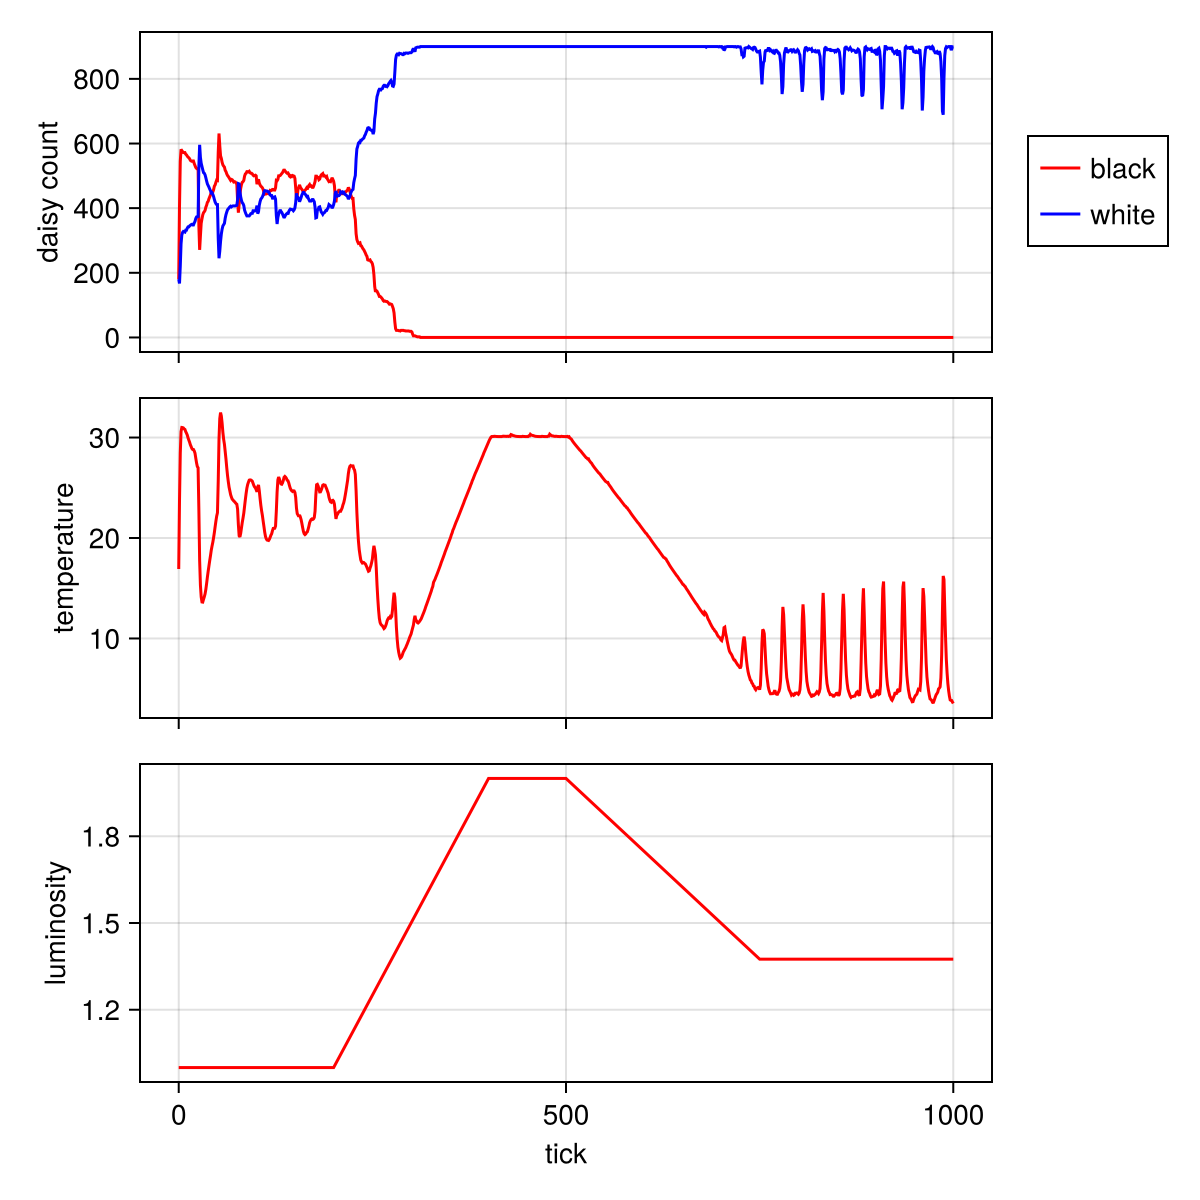
\includegraphics[width=0.7\linewidth,height=\textheight,keepaspectratio]{image/daisy_luminosity.png}

}

\caption{\label{fig-luminosity}Динамика модели при изменении светимости}

\end{figure}%

\section{Параметрическое
исследование}\label{ux43fux430ux440ux430ux43cux435ux442ux440ux438ux447ux435ux441ux43aux43eux435-ux438ux441ux441ux43bux435ux434ux43eux432ux430ux43dux438ux435}

Для исследования влияния параметров были созданы три скрипта с
параметрическими запусками (рис. Рисунок~\ref{fig-param}):

\begin{itemize}
\tightlist
\item
  \texttt{daisyworld\_\_param\_lit.jl} -- базовая визуализация для
  комбинаций \texttt{max\_age} и \texttt{init\_white}.
\item
  \texttt{daisyworld-count\_\_param\_lit.jl} -- графики численности.
\item
  \texttt{daisyworld-luminosity\_\_param\_lit.jl} -- комплексные графики
  для сценария \texttt{:ramp}.
\end{itemize}

\begin{figure}

\centering{


\includegraphics[width=0.7\linewidth,height=\textheight,keepaspectratio]{image/6.png}

}

\caption{\label{fig-param}Параметрические запуски в терминале}

\end{figure}%

Пример результатов параметрического исследования показан на рис.
Рисунок~\ref{fig-param-count}.

\begin{figure}

\centering{

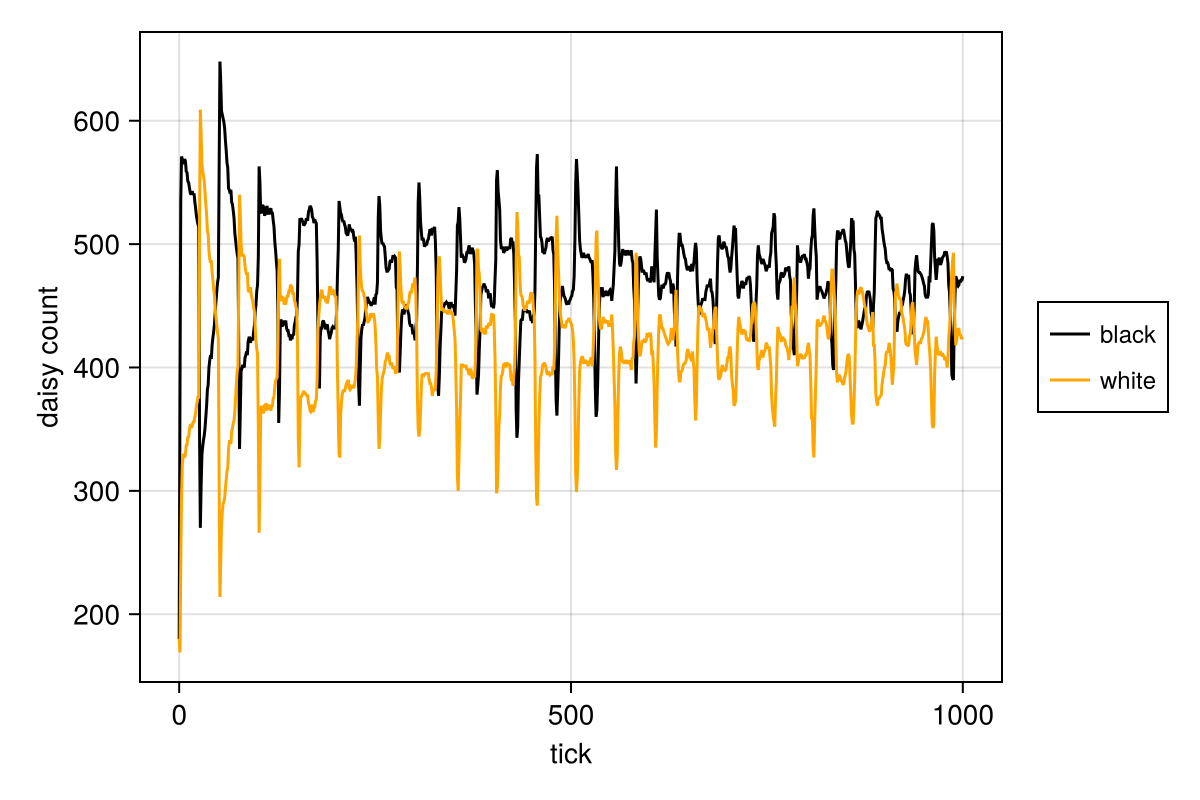
\includegraphics[width=0.7\linewidth,height=\textheight,keepaspectratio]{image/daisy-count_maxage=25_initwhite=0.2.png}

}

\caption{\label{fig-param-count}Графики численности для разных
параметров}

\end{figure}%

\section{Генерация производных
форматов}\label{ux433ux435ux43dux435ux440ux430ux446ux438ux44f-ux43fux440ux43eux438ux437ux432ux43eux434ux43dux44bux445-ux444ux43eux440ux43cux430ux442ux43eux432}

С помощью скрипта \texttt{scripts/tangle.jl} для каждого литературного
скрипта были созданы чистый код, Jupyter Notebook и документ Quarto
(рис. Рисунок~\ref{fig-tangle}). Эти файлы сохранены в
\texttt{labs/project/scripts}, \texttt{labs/project/markdown},
\texttt{labs/project/notebooks}.

\begin{figure}

\centering{


\includegraphics[width=0.7\linewidth,height=\textheight,keepaspectratio]{image/4.png}

}

\caption{\label{fig-tangle}Генерация производных форматов для
\texttt{daisyworld\_lit.jl}}

\end{figure}%

\begin{figure}

\centering{


\includegraphics[width=0.7\linewidth,height=\textheight,keepaspectratio]{image/5.png}

}

\caption{\label{fig-generated}Содержимое папок после генерации}

\end{figure}%

\section{Интеграция в
отчёт}\label{ux438ux43dux442ux435ux433ux440ux430ux446ux438ux44f-ux432-ux43eux442ux447ux451ux442}

Все сгенерированные Quarto-документы были включены в отчёт с помощью
конструкции \texttt{\{\{\textless{}\ include\ \textgreater{}\}\}} (см.
раздел \textbf{Реализация}).

\chapter{Реализация}\label{ux440ux435ux430ux43bux438ux437ux430ux446ux438ux44f}

\section{Базовая
модель}\label{ux431ux430ux437ux43eux432ux430ux44f-ux43cux43eux434ux435ux43bux44c}

\subsection{Базовая визуализация
Daisyworld}\label{ux431ux430ux437ux43eux432ux430ux44f-ux432ux438ux437ux443ux430ux43bux438ux437ux430ux446ux438ux44f-daisyworld}

Создадим модель и отобразим её состояние на нескольких шагах: начальное,
после 5 шагов и после 40 шагов. Используется тепловая карта температуры,
маргаритки отображаются символами.

\subsubsection{Инициализация (проект активирован через командную
строку)}\label{ux438ux43dux438ux446ux438ux430ux43bux438ux437ux430ux446ux438ux44f-ux43fux440ux43eux435ux43aux442-ux430ux43aux442ux438ux432ux438ux440ux43eux432ux430ux43d-ux447ux435ux440ux435ux437-ux43aux43eux43cux430ux43dux434ux43dux443ux44e-ux441ux442ux440ux43eux43aux443}

\begin{Shaded}
\begin{Highlighting}[]
\ImportTok{using} \BuiltInTok{DrWatson}
\ImportTok{using} \BuiltInTok{Agents}
\ImportTok{using} \BuiltInTok{CairoMakie}
\ImportTok{using} \BuiltInTok{Plots}
\end{Highlighting}
\end{Shaded}

Подключаем определение модели (относительный путь от скрипта)

\begin{Shaded}
\begin{Highlighting}[]
\FunctionTok{include}\NormalTok{(}\FunctionTok{joinpath}\NormalTok{(}\PreprocessorTok{@\_\_DIR\_\_}\NormalTok{, }\StringTok{".."}\NormalTok{, }\StringTok{"src"}\NormalTok{, }\StringTok{"daisyworld.jl"}\NormalTok{))}
\end{Highlighting}
\end{Shaded}

\begin{verbatim}
daisyworld (generic function with 1 method)
\end{verbatim}

\subsubsection{Настройки
визуализации}\label{ux43dux430ux441ux442ux440ux43eux439ux43aux438-ux432ux438ux437ux443ux430ux43bux438ux437ux430ux446ux438ux438}

\begin{Shaded}
\begin{Highlighting}[]
\FunctionTok{daisycolor}\NormalTok{(a}\OperatorTok{::}\DataTypeTok{Daisy}\NormalTok{) }\OperatorTok{=}\NormalTok{ a.breed}

\NormalTok{plotkwargs }\OperatorTok{=}\NormalTok{ (}
\NormalTok{    agent\_color }\OperatorTok{=}\NormalTok{ daisycolor,}
\NormalTok{    agent\_size }\OperatorTok{=} \FloatTok{20}\NormalTok{,}
\NormalTok{    agent\_marker }\OperatorTok{=} \CharTok{\textquotesingle{}✿\textquotesingle{}}\NormalTok{,}
\NormalTok{    heatarray }\OperatorTok{=} \OperatorTok{:}\NormalTok{temperature,}
\NormalTok{    heatkwargs }\OperatorTok{=}\NormalTok{ (colorrange }\OperatorTok{=}\NormalTok{ (}\OperatorTok{{-}}\FloatTok{20}\NormalTok{, }\FloatTok{60}\NormalTok{),),}
\NormalTok{)}
\end{Highlighting}
\end{Shaded}

\begin{verbatim}
(agent_color = Main.Notebook.daisycolor, agent_size = 20, agent_marker = '✿', heatarray = :temperature, heatkwargs = (colorrange = (-20, 60),))
\end{verbatim}

\subsubsection{Запуск и сохранение
кадров}\label{ux437ux430ux43fux443ux441ux43a-ux438-ux441ux43eux445ux440ux430ux43dux435ux43dux438ux435-ux43aux430ux434ux440ux43eux432}

\begin{Shaded}
\begin{Highlighting}[]
\NormalTok{model }\OperatorTok{=} \FunctionTok{daisyworld}\NormalTok{()}

\NormalTok{plt1, \_ }\OperatorTok{=} \FunctionTok{abmplot}\NormalTok{(model; plotkwargs}\OperatorTok{...}\NormalTok{)}
\FunctionTok{display}\NormalTok{(plt1)  }\CommentTok{\# \textless{}{-}{-} добавлено}

\FunctionTok{step!}\NormalTok{(model, }\FloatTok{5}\NormalTok{)}
\NormalTok{plt2, \_ }\OperatorTok{=} \FunctionTok{abmplot}\NormalTok{(model; heatarray }\OperatorTok{=}\NormalTok{ model.temperature, plotkwargs}\OperatorTok{...}\NormalTok{)}
\FunctionTok{display}\NormalTok{(plt2)  }\CommentTok{\# \textless{}{-}{-} добавлено}

\FunctionTok{step!}\NormalTok{(model, }\FloatTok{35}\NormalTok{)  }\CommentTok{\# итого 40}
\NormalTok{plt3, \_ }\OperatorTok{=} \FunctionTok{abmplot}\NormalTok{(model; heatarray }\OperatorTok{=}\NormalTok{ model.temperature, plotkwargs}\OperatorTok{...}\NormalTok{)}
\FunctionTok{display}\NormalTok{(plt3)  }\CommentTok{\# \textless{}{-}{-} добавлено}
\end{Highlighting}
\end{Shaded}

\pandocbounded{
\includegraphics[keepaspectratio]{simulation-modeling-lab03-report_files/mediabag/simulation-modeling-lab03-report_files/figure-pdf/cell-5-output-1.pdf}}

\pandocbounded{\includegraphics[keepaspectratio]{simulation-modeling-lab03-report_files/mediabag/simulation-modeling-lab03-report_files/figure-pdf/cell-5-output-2.pdf}}

\pandocbounded{\includegraphics[keepaspectratio]{simulation-modeling-lab03-report_files/mediabag/simulation-modeling-lab03-report_files/figure-pdf/cell-5-output-3.pdf}}

\begin{verbatim}
CairoMakie.Screen{PDF}
\end{verbatim}

Сохраняем графики в папку \texttt{plots} на уровне выше скрипта

\begin{Shaded}
\begin{Highlighting}[]
\NormalTok{plots\_dir }\OperatorTok{=} \FunctionTok{joinpath}\NormalTok{(}\PreprocessorTok{@\_\_DIR\_\_}\NormalTok{, }\StringTok{".."}\NormalTok{, }\StringTok{"plots"}\NormalTok{)}
\FunctionTok{mkpath}\NormalTok{(plots\_dir)}

\FunctionTok{save}\NormalTok{(}\FunctionTok{joinpath}\NormalTok{(plots\_dir, }\StringTok{"daisy\_step001.png"}\NormalTok{), plt1)}
\FunctionTok{save}\NormalTok{(}\FunctionTok{joinpath}\NormalTok{(plots\_dir, }\StringTok{"daisy\_step005.png"}\NormalTok{), plt2)}
\FunctionTok{save}\NormalTok{(}\FunctionTok{joinpath}\NormalTok{(plots\_dir, }\StringTok{"daisy\_step040.png"}\NormalTok{), plt3)}

\FunctionTok{println}\NormalTok{(}\StringTok{"Графики сохранены в }\SpecialCharTok{$}\NormalTok{plots\_dir}\StringTok{"}\NormalTok{)}
\end{Highlighting}
\end{Shaded}

\begin{verbatim}
Графики сохранены в /home/vvmalyuga/work/study/2026-1/2026-1--study--simulation-modeling/labs/lab03/report/../plots
\end{verbatim}

\section{Анимация}\label{ux430ux43dux438ux43cux430ux446ux438ux44f-1}

\subsection{Анимация модели
Daisyworld}\label{ux430ux43dux438ux43cux430ux446ux438ux44f-ux43cux43eux434ux435ux43bux438-daisyworld}

\begin{Shaded}
\begin{Highlighting}[]
\ImportTok{using} \BuiltInTok{DrWatson}
\ImportTok{using} \BuiltInTok{Agents}
\ImportTok{using} \BuiltInTok{CairoMakie}

\FunctionTok{include}\NormalTok{(}\FunctionTok{joinpath}\NormalTok{(}\PreprocessorTok{@\_\_DIR\_\_}\NormalTok{, }\StringTok{".."}\NormalTok{, }\StringTok{"src"}\NormalTok{, }\StringTok{"daisyworld.jl"}\NormalTok{))}

\FunctionTok{daisycolor}\NormalTok{(a}\OperatorTok{::}\DataTypeTok{Daisy}\NormalTok{) }\OperatorTok{=}\NormalTok{ a.breed}

\NormalTok{plotkwargs }\OperatorTok{=}\NormalTok{ (}
\NormalTok{    agent\_color }\OperatorTok{=}\NormalTok{ daisycolor,}
\NormalTok{    agent\_size }\OperatorTok{=} \FloatTok{20}\NormalTok{,}
\NormalTok{    agent\_marker }\OperatorTok{=} \CharTok{\textquotesingle{}✿\textquotesingle{}}\NormalTok{,}
\NormalTok{    heatarray }\OperatorTok{=} \OperatorTok{:}\NormalTok{temperature,}
\NormalTok{    heatkwargs }\OperatorTok{=}\NormalTok{ (colorrange }\OperatorTok{=}\NormalTok{ (}\OperatorTok{{-}}\FloatTok{20}\NormalTok{, }\FloatTok{60}\NormalTok{),),}
\NormalTok{)}

\NormalTok{model }\OperatorTok{=} \FunctionTok{daisyworld}\NormalTok{()}

\NormalTok{plots\_dir }\OperatorTok{=} \FunctionTok{joinpath}\NormalTok{(}\PreprocessorTok{@\_\_DIR\_\_}\NormalTok{, }\StringTok{".."}\NormalTok{, }\StringTok{"plots"}\NormalTok{)}
\FunctionTok{mkpath}\NormalTok{(plots\_dir)}

\FunctionTok{abmvideo}\NormalTok{(}
    \FunctionTok{joinpath}\NormalTok{(plots\_dir, }\StringTok{"simulation.webm"}\NormalTok{),}
\NormalTok{    model;}
\NormalTok{    title }\OperatorTok{=} \StringTok{"Daisy World"}\NormalTok{,}
\NormalTok{    frames }\OperatorTok{=} \FloatTok{60}\NormalTok{,}
\NormalTok{    plotkwargs}\OperatorTok{...}\NormalTok{,}
\NormalTok{)}
\FunctionTok{println}\NormalTok{(}\StringTok{"Видео сохранено в }\SpecialCharTok{$}\NormalTok{plots\_dir}\StringTok{/simulation.mp4"}\NormalTok{)}
\end{Highlighting}
\end{Shaded}

\begin{verbatim}
Видео сохранено в /home/vvmalyuga/work/study/2026-1/2026-1--study--simulation-modeling/labs/lab03/report/../plots/simulation.mp4
\end{verbatim}

\section{Динамика
численности}\label{ux434ux438ux43dux430ux43cux438ux43aux430-ux447ux438ux441ux43bux435ux43dux43dux43eux441ux442ux438-1}

\subsection{Динамика численности
маргариток}\label{ux434ux438ux43dux430ux43cux438ux43aux430-ux447ux438ux441ux43bux435ux43dux43dux43eux441ux442ux438-ux43cux430ux440ux433ux430ux440ux438ux442ux43eux43a}

\begin{Shaded}
\begin{Highlighting}[]
\ImportTok{using} \BuiltInTok{DrWatson}
\ImportTok{using} \BuiltInTok{Agents}
\ImportTok{using} \BuiltInTok{CairoMakie}
\ImportTok{using} \BuiltInTok{DataFrames}

\FunctionTok{include}\NormalTok{(}\FunctionTok{joinpath}\NormalTok{(}\PreprocessorTok{@\_\_DIR\_\_}\NormalTok{, }\StringTok{".."}\NormalTok{, }\StringTok{"src"}\NormalTok{, }\StringTok{"daisyworld.jl"}\NormalTok{))}

\FunctionTok{black}\NormalTok{(a) }\OperatorTok{=}\NormalTok{ a.breed }\OperatorTok{==} \OperatorTok{:}\NormalTok{black}
\FunctionTok{white}\NormalTok{(a) }\OperatorTok{=}\NormalTok{ a.breed }\OperatorTok{==} \OperatorTok{:}\NormalTok{white}
\NormalTok{adata }\OperatorTok{=}\NormalTok{ [(black, count), (white, count)]}

\NormalTok{model }\OperatorTok{=} \FunctionTok{daisyworld}\NormalTok{(; solar\_luminosity }\OperatorTok{=} \FloatTok{1.0}\NormalTok{)}
\NormalTok{agent\_df, model\_df }\OperatorTok{=} \FunctionTok{run!}\NormalTok{(model, }\FloatTok{1000}\NormalTok{; adata)}

\NormalTok{figure }\OperatorTok{=} \FunctionTok{Figure}\NormalTok{(size }\OperatorTok{=}\NormalTok{ (}\FloatTok{600}\NormalTok{, }\FloatTok{400}\NormalTok{))}
\NormalTok{ax }\OperatorTok{=} \FunctionTok{Axis}\NormalTok{(figure[}\FloatTok{1}\NormalTok{, }\FloatTok{1}\NormalTok{], xlabel }\OperatorTok{=} \StringTok{"tick"}\NormalTok{, ylabel }\OperatorTok{=} \StringTok{"daisy count"}\NormalTok{)}

\NormalTok{blackl }\OperatorTok{=} \FunctionTok{lines!}\NormalTok{(ax, agent\_df[!, }\OperatorTok{:}\NormalTok{time], agent\_df[!, }\OperatorTok{:}\NormalTok{count\_black], color }\OperatorTok{=} \OperatorTok{:}\NormalTok{black)}
\NormalTok{whitel }\OperatorTok{=} \FunctionTok{lines!}\NormalTok{(ax, agent\_df[!, }\OperatorTok{:}\NormalTok{time], agent\_df[!, }\OperatorTok{:}\NormalTok{count\_white], color }\OperatorTok{=} \OperatorTok{:}\NormalTok{orange)}

\FunctionTok{Legend}\NormalTok{(figure[}\FloatTok{1}\NormalTok{, }\FloatTok{2}\NormalTok{], [blackl, whitel], [}\StringTok{"black"}\NormalTok{, }\StringTok{"white"}\NormalTok{], labelsize }\OperatorTok{=} \FloatTok{12}\NormalTok{)}
\FunctionTok{display}\NormalTok{(figure)  }\CommentTok{\# \textless{}{-}{-} добавлено}

\NormalTok{plots\_dir }\OperatorTok{=} \FunctionTok{joinpath}\NormalTok{(}\PreprocessorTok{@\_\_DIR\_\_}\NormalTok{, }\StringTok{".."}\NormalTok{, }\StringTok{"plots"}\NormalTok{)}
\FunctionTok{mkpath}\NormalTok{(plots\_dir)}
\FunctionTok{save}\NormalTok{(}\FunctionTok{joinpath}\NormalTok{(plots\_dir, }\StringTok{"daisy\_count.png"}\NormalTok{), figure)}

\FunctionTok{println}\NormalTok{(}\StringTok{"График численности сохранён в }\SpecialCharTok{$}\NormalTok{plots\_dir}\StringTok{/daisy\_count.png"}\NormalTok{)}
\end{Highlighting}
\end{Shaded}

\begin{verbatim}
График численности сохранён в /home/vvmalyuga/work/study/2026-1/2026-1--study--simulation-modeling/labs/lab03/report/../plots/daisy_count.png
\end{verbatim}

\pandocbounded{
\includegraphics[keepaspectratio]{simulation-modeling-lab03-report_files/mediabag/simulation-modeling-lab03-report_files/figure-pdf/cell-8-output-2.pdf}}

\section{Динамика при изменении
светимости}\label{ux434ux438ux43dux430ux43cux438ux43aux430-ux43fux440ux438-ux438ux437ux43cux435ux43dux435ux43dux438ux438-ux441ux432ux435ux442ux438ux43cux43eux441ux442ux438}

\subsection{Динамика модели при изменении солнечной
активности}\label{ux434ux438ux43dux430ux43cux438ux43aux430-ux43cux43eux434ux435ux43bux438-ux43fux440ux438-ux438ux437ux43cux435ux43dux435ux43dux438ux438-ux441ux43eux43bux43dux435ux447ux43dux43eux439-ux430ux43aux442ux438ux432ux43dux43eux441ux442ux438}

Используем сценарий \texttt{:ramp}, при котором светимость сначала
увеличивается, а затем уменьшается. Строим графики численности
маргариток, средней температуры и светимости.

\begin{Shaded}
\begin{Highlighting}[]
\ImportTok{using} \BuiltInTok{DrWatson}
\ImportTok{using} \BuiltInTok{Agents}
\ImportTok{using} \BuiltInTok{CairoMakie}
\ImportTok{using} \BuiltInTok{DataFrames}
\ImportTok{using} \BuiltInTok{StatsBase}

\FunctionTok{include}\NormalTok{(}\FunctionTok{joinpath}\NormalTok{(}\PreprocessorTok{@\_\_DIR\_\_}\NormalTok{, }\StringTok{".."}\NormalTok{, }\StringTok{"src"}\NormalTok{, }\StringTok{"daisyworld.jl"}\NormalTok{))}
\end{Highlighting}
\end{Shaded}

\begin{verbatim}
daisyworld (generic function with 1 method)
\end{verbatim}

\subsubsection{Агрегаторы}\label{ux430ux433ux440ux435ux433ux430ux442ux43eux440ux44b}

\begin{Shaded}
\begin{Highlighting}[]
\FunctionTok{black}\NormalTok{(a) }\OperatorTok{=}\NormalTok{ a.breed }\OperatorTok{==} \OperatorTok{:}\NormalTok{black}
\FunctionTok{white}\NormalTok{(a) }\OperatorTok{=}\NormalTok{ a.breed }\OperatorTok{==} \OperatorTok{:}\NormalTok{white}
\NormalTok{adata }\OperatorTok{=}\NormalTok{ [(black, count), (white, count)]}
\end{Highlighting}
\end{Shaded}

\begin{verbatim}
2-element Vector{Tuple{Function, typeof(count)}}:
 (Main.Notebook.black, count)
 (Main.Notebook.white, count)
\end{verbatim}

\subsubsection{Запуск модели со сценарием
:ramp}\label{ux437ux430ux43fux443ux441ux43a-ux43cux43eux434ux435ux43bux438-ux441ux43e-ux441ux446ux435ux43dux430ux440ux438ux435ux43c-ramp}

\begin{Shaded}
\begin{Highlighting}[]
\NormalTok{model }\OperatorTok{=} \FunctionTok{daisyworld}\NormalTok{(solar\_luminosity }\OperatorTok{=} \FloatTok{1.0}\NormalTok{, scenario }\OperatorTok{=} \OperatorTok{:}\NormalTok{ramp)}

\FunctionTok{temperature}\NormalTok{(model) }\OperatorTok{=}\NormalTok{ StatsBase.}\FunctionTok{mean}\NormalTok{(model.temperature)}
\NormalTok{mdata }\OperatorTok{=}\NormalTok{ [temperature, }\OperatorTok{:}\NormalTok{solar\_luminosity]}

\NormalTok{agent\_df, model\_df }\OperatorTok{=} \FunctionTok{run!}\NormalTok{(model, }\FloatTok{1000}\NormalTok{; adata }\OperatorTok{=}\NormalTok{ adata, mdata }\OperatorTok{=}\NormalTok{ mdata)}

\NormalTok{figure }\OperatorTok{=}\NormalTok{ CairoMakie.}\FunctionTok{Figure}\NormalTok{(size }\OperatorTok{=}\NormalTok{ (}\FloatTok{600}\NormalTok{, }\FloatTok{600}\NormalTok{))}

\NormalTok{ax1 }\OperatorTok{=} \FunctionTok{Axis}\NormalTok{(figure[}\FloatTok{1}\NormalTok{, }\FloatTok{1}\NormalTok{], ylabel }\OperatorTok{=} \StringTok{"daisy count"}\NormalTok{)}
\NormalTok{blackl }\OperatorTok{=} \FunctionTok{lines!}\NormalTok{(ax1, agent\_df[!, }\OperatorTok{:}\NormalTok{time], agent\_df[!, }\OperatorTok{:}\NormalTok{count\_black], color }\OperatorTok{=} \OperatorTok{:}\NormalTok{red)}
\NormalTok{whitel }\OperatorTok{=} \FunctionTok{lines!}\NormalTok{(ax1, agent\_df[!, }\OperatorTok{:}\NormalTok{time], agent\_df[!, }\OperatorTok{:}\NormalTok{count\_white], color }\OperatorTok{=} \OperatorTok{:}\NormalTok{blue)}
\NormalTok{figure[}\FloatTok{1}\NormalTok{, }\FloatTok{2}\NormalTok{] }\OperatorTok{=} \FunctionTok{Legend}\NormalTok{(figure, [blackl, whitel], [}\StringTok{"black"}\NormalTok{, }\StringTok{"white"}\NormalTok{])}

\NormalTok{ax2 }\OperatorTok{=} \FunctionTok{Axis}\NormalTok{(figure[}\FloatTok{2}\NormalTok{, }\FloatTok{1}\NormalTok{], ylabel }\OperatorTok{=} \StringTok{"temperature"}\NormalTok{)}
\FunctionTok{lines!}\NormalTok{(ax2, model\_df[!, }\OperatorTok{:}\NormalTok{time], model\_df[!, }\OperatorTok{:}\NormalTok{temperature], color }\OperatorTok{=} \OperatorTok{:}\NormalTok{red)}

\NormalTok{ax3 }\OperatorTok{=} \FunctionTok{Axis}\NormalTok{(figure[}\FloatTok{3}\NormalTok{, }\FloatTok{1}\NormalTok{], xlabel }\OperatorTok{=} \StringTok{"tick"}\NormalTok{, ylabel }\OperatorTok{=} \StringTok{"luminosity"}\NormalTok{)}
\FunctionTok{lines!}\NormalTok{(ax3, model\_df[!, }\OperatorTok{:}\NormalTok{time], model\_df[!, }\OperatorTok{:}\NormalTok{solar\_luminosity], color }\OperatorTok{=} \OperatorTok{:}\NormalTok{red)}

\ControlFlowTok{for}\NormalTok{ ax }\KeywordTok{in}\NormalTok{ (ax1, ax2)}
\NormalTok{    ax.xticklabelsvisible }\OperatorTok{=} \ConstantTok{false}
\ControlFlowTok{end}

\CommentTok{\# Отображаем график}
\FunctionTok{display}\NormalTok{(figure)}

\NormalTok{plots\_dir }\OperatorTok{=} \FunctionTok{plotsdir}\NormalTok{()}
\FunctionTok{mkpath}\NormalTok{(plots\_dir)}
\FunctionTok{save}\NormalTok{(}\FunctionTok{joinpath}\NormalTok{(plots\_dir, }\StringTok{"daisy\_luminosity.png"}\NormalTok{), figure)}

\FunctionTok{println}\NormalTok{(}\StringTok{"График динамики сохранён в }\SpecialCharTok{$}\NormalTok{plots\_dir}\StringTok{/daisy\_luminosity.png"}\NormalTok{)}
\end{Highlighting}
\end{Shaded}

\begin{verbatim}
График динамики сохранён в /home/vvmalyuga/work/study/2026-1/2026-1--study--simulation-modeling/labs/project/plots/daisy_luminosity.png
\end{verbatim}

\pandocbounded{
\includegraphics[keepaspectratio]{simulation-modeling-lab03-report_files/mediabag/simulation-modeling-lab03-report_files/figure-pdf/cell-11-output-2.pdf}}

\section{Параметрическое исследование (базовая
визуализация)}\label{ux43fux430ux440ux430ux43cux435ux442ux440ux438ux447ux435ux441ux43aux43eux435-ux438ux441ux441ux43bux435ux434ux43eux432ux430ux43dux438ux435-ux431ux430ux437ux43eux432ux430ux44f-ux432ux438ux437ux443ux430ux43bux438ux437ux430ux446ux438ux44f}

\subsection{Параметрическое исследование: базовая
визуализация}\label{ux43fux430ux440ux430ux43cux435ux442ux440ux438ux447ux435ux441ux43aux43eux435-ux438ux441ux441ux43bux435ux434ux43eux432ux430ux43dux438ux435-ux431ux430ux437ux43eux432ux430ux44f-ux432ux438ux437ux443ux430ux43bux438ux437ux430ux446ux438ux44f-1}

Исследуем влияние максимального возраста (\texttt{max\_age}) и начальной
доли белых маргариток (\texttt{init\_white}) на визуальную картину
модели.

\begin{Shaded}
\begin{Highlighting}[]
\ImportTok{using} \BuiltInTok{DrWatson}
\ImportTok{using} \BuiltInTok{Agents}
\ImportTok{using} \BuiltInTok{CairoMakie}
\ImportTok{using} \BuiltInTok{DataFrames}

\FunctionTok{include}\NormalTok{(}\FunctionTok{joinpath}\NormalTok{(}\PreprocessorTok{@\_\_DIR\_\_}\NormalTok{, }\StringTok{".."}\NormalTok{, }\StringTok{"src"}\NormalTok{, }\StringTok{"daisyworld.jl"}\NormalTok{))}
\end{Highlighting}
\end{Shaded}

\begin{verbatim}
daisyworld (generic function with 1 method)
\end{verbatim}

\subsubsection{Параметры
эксперимента}\label{ux43fux430ux440ux430ux43cux435ux442ux440ux44b-ux44dux43aux441ux43fux435ux440ux438ux43cux435ux43dux442ux430}

\begin{Shaded}
\begin{Highlighting}[]
\NormalTok{param\_dict }\OperatorTok{=} \FunctionTok{Dict}\NormalTok{(}
    \OperatorTok{:}\NormalTok{griddims }\OperatorTok{=\textgreater{}}\NormalTok{ (}\FloatTok{30}\NormalTok{, }\FloatTok{30}\NormalTok{),}
    \OperatorTok{:}\NormalTok{max\_age }\OperatorTok{=\textgreater{}}\NormalTok{ [}\FloatTok{25}\NormalTok{, }\FloatTok{40}\NormalTok{],}
    \OperatorTok{:}\NormalTok{init\_white }\OperatorTok{=\textgreater{}}\NormalTok{ [}\FloatTok{0.2}\NormalTok{, }\FloatTok{0.8}\NormalTok{],}
    \OperatorTok{:}\NormalTok{init\_black }\OperatorTok{=\textgreater{}} \FloatTok{0.2}\NormalTok{,}
    \OperatorTok{:}\NormalTok{albedo\_white }\OperatorTok{=\textgreater{}} \FloatTok{0.75}\NormalTok{,}
    \OperatorTok{:}\NormalTok{albedo\_black }\OperatorTok{=\textgreater{}} \FloatTok{0.25}\NormalTok{,}
    \OperatorTok{:}\NormalTok{surface\_albedo }\OperatorTok{=\textgreater{}} \FloatTok{0.4}\NormalTok{,}
    \OperatorTok{:}\NormalTok{solar\_change }\OperatorTok{=\textgreater{}} \FloatTok{0.005}\NormalTok{,}
    \OperatorTok{:}\NormalTok{solar\_luminosity }\OperatorTok{=\textgreater{}} \FloatTok{1.0}\NormalTok{,}
    \OperatorTok{:}\NormalTok{scenario }\OperatorTok{=\textgreater{}} \OperatorTok{:}\NormalTok{default,}
    \OperatorTok{:}\NormalTok{seed }\OperatorTok{=\textgreater{}} \FloatTok{165}\NormalTok{,}
\NormalTok{)}
\end{Highlighting}
\end{Shaded}

\begin{verbatim}
Dict{Symbol, Any} with 11 entries:
  :solar_luminosity => 1.0
  :scenario         => :default
  :griddims         => (30, 30)
  :max_age          => [25, 40]
  :surface_albedo   => 0.4
  :init_white       => [0.2, 0.8]
  :albedo_white     => 0.75
  :init_black       => 0.2
  :solar_change     => 0.005
  :albedo_black     => 0.25
  :seed             => 165
\end{verbatim}

Генерируем все комбинации

\begin{Shaded}
\begin{Highlighting}[]
\NormalTok{params\_list }\OperatorTok{=} \FunctionTok{dict\_list}\NormalTok{(param\_dict)}

\NormalTok{plots\_dir }\OperatorTok{=} \FunctionTok{joinpath}\NormalTok{(}\PreprocessorTok{@\_\_DIR\_\_}\NormalTok{, }\StringTok{".."}\NormalTok{, }\StringTok{"plots"}\NormalTok{)}
\FunctionTok{mkpath}\NormalTok{(plots\_dir)}

\ControlFlowTok{for}\NormalTok{ params }\KeywordTok{in}\NormalTok{ params\_list}
    \KeywordTok{global}\NormalTok{ current\_params }\OperatorTok{=}\NormalTok{ params}
\NormalTok{    model }\OperatorTok{=} \FunctionTok{daisyworld}\NormalTok{(; params}\OperatorTok{...}\NormalTok{)}

    \FunctionTok{daisycolor}\NormalTok{(a}\OperatorTok{::}\DataTypeTok{Daisy}\NormalTok{) }\OperatorTok{=}\NormalTok{ a.breed}

\NormalTok{    plotkwargs }\OperatorTok{=}\NormalTok{ (}
\NormalTok{        agent\_color }\OperatorTok{=}\NormalTok{ daisycolor,}
\NormalTok{        agent\_size }\OperatorTok{=} \FloatTok{20}\NormalTok{,}
\NormalTok{        agent\_marker }\OperatorTok{=} \CharTok{\textquotesingle{}✿\textquotesingle{}}\NormalTok{,}
\NormalTok{        heatarray }\OperatorTok{=} \OperatorTok{:}\NormalTok{temperature,}
\NormalTok{        heatkwargs }\OperatorTok{=}\NormalTok{ (colorrange }\OperatorTok{=}\NormalTok{ (}\OperatorTok{{-}}\FloatTok{20}\NormalTok{, }\FloatTok{60}\NormalTok{),),}
\NormalTok{    )}
    
\ControlFlowTok{end}
\end{Highlighting}
\end{Shaded}

Шаг 0

\begin{Shaded}
\begin{Highlighting}[]
\NormalTok{    plt1, \_ }\OperatorTok{=} \FunctionTok{abmplot}\NormalTok{(model; plotkwargs}\OperatorTok{...}\NormalTok{)}
    \FunctionTok{display}\NormalTok{(figure)  }\CommentTok{\# \textless{}{-}{-} добавлено}
\end{Highlighting}
\end{Shaded}

\pandocbounded{
\includegraphics[keepaspectratio]{simulation-modeling-lab03-report_files/mediabag/simulation-modeling-lab03-report_files/figure-pdf/cell-15-output-1.pdf}}

\begin{verbatim}
CairoMakie.Screen{PDF}
\end{verbatim}

Шаг 5

\begin{Shaded}
\begin{Highlighting}[]
    \FunctionTok{step!}\NormalTok{(model, }\FloatTok{5}\NormalTok{)}
\NormalTok{    plt2, \_ }\OperatorTok{=} \FunctionTok{abmplot}\NormalTok{(model; heatarray }\OperatorTok{=}\NormalTok{ model.temperature, plotkwargs}\OperatorTok{...}\NormalTok{)}
    \FunctionTok{display}\NormalTok{(figure)  }\CommentTok{\# \textless{}{-}{-} добавлено}
\end{Highlighting}
\end{Shaded}

\pandocbounded{
\includegraphics[keepaspectratio]{simulation-modeling-lab03-report_files/mediabag/simulation-modeling-lab03-report_files/figure-pdf/cell-16-output-1.pdf}}

\begin{verbatim}
CairoMakie.Screen{PDF}
\end{verbatim}

Шаг 40

\begin{Shaded}
\begin{Highlighting}[]
    \FunctionTok{step!}\NormalTok{(model, }\FloatTok{35}\NormalTok{)}
\NormalTok{    plt3, \_ }\OperatorTok{=} \FunctionTok{abmplot}\NormalTok{(model; heatarray }\OperatorTok{=}\NormalTok{ model.temperature, plotkwargs}\OperatorTok{...}\NormalTok{)}
    \FunctionTok{display}\NormalTok{(figure)  }\CommentTok{\# \textless{}{-}{-} добавлено}
\end{Highlighting}
\end{Shaded}

\pandocbounded{
\includegraphics[keepaspectratio]{simulation-modeling-lab03-report_files/mediabag/simulation-modeling-lab03-report_files/figure-pdf/cell-17-output-1.pdf}}

\begin{verbatim}
CairoMakie.Screen{PDF}
\end{verbatim}

Формируем имена файлов с параметрами

\begin{Shaded}
\begin{Highlighting}[]
\CommentTok{\#\#\#\# Сохраняем}
\NormalTok{    prefix }\OperatorTok{=} \FunctionTok{savename}\NormalTok{(}\StringTok{"daisyworld"}\NormalTok{, current\_params)}
    \FunctionTok{save}\NormalTok{(}\FunctionTok{joinpath}\NormalTok{(plots\_dir, prefix }\OperatorTok{*} \StringTok{"\_step01.png"}\NormalTok{), plt1)}
    \FunctionTok{save}\NormalTok{(}\FunctionTok{joinpath}\NormalTok{(plots\_dir, prefix }\OperatorTok{*} \StringTok{"\_step05.png"}\NormalTok{), plt2)}
    \FunctionTok{save}\NormalTok{(}\FunctionTok{joinpath}\NormalTok{(plots\_dir, prefix }\OperatorTok{*} \StringTok{"\_step40.png"}\NormalTok{), plt3)}

\FunctionTok{println}\NormalTok{(}\StringTok{"Все параметрические кадры сохранены в }\SpecialCharTok{$}\NormalTok{plots\_dir}\StringTok{"}\NormalTok{)}
\end{Highlighting}
\end{Shaded}

\begin{verbatim}
Все параметрические кадры сохранены в /home/vvmalyuga/work/study/2026-1/2026-1--study--simulation-modeling/labs/lab03/report/../plots
\end{verbatim}

\section{Параметрическое исследование (динамика
численности)}\label{ux43fux430ux440ux430ux43cux435ux442ux440ux438ux447ux435ux441ux43aux43eux435-ux438ux441ux441ux43bux435ux434ux43eux432ux430ux43dux438ux435-ux434ux438ux43dux430ux43cux438ux43aux430-ux447ux438ux441ux43bux435ux43dux43dux43eux441ux442ux438}

\subsection{Параметрическое исследование: динамика
численности}\label{ux43fux430ux440ux430ux43cux435ux442ux440ux438ux447ux435ux441ux43aux43eux435-ux438ux441ux441ux43bux435ux434ux43eux432ux430ux43dux438ux435-ux434ux438ux43dux430ux43cux438ux43aux430-ux447ux438ux441ux43bux435ux43dux43dux43eux441ux442ux438-1}

Для тех же комбинаций параметров (max\_age, init\_white) строим графики
изменения числа маргариток во времени.

\begin{Shaded}
\begin{Highlighting}[]
\ImportTok{using} \BuiltInTok{DrWatson}
\ImportTok{using} \BuiltInTok{Agents}
\ImportTok{using} \BuiltInTok{CairoMakie}
\ImportTok{using} \BuiltInTok{DataFrames}

\FunctionTok{include}\NormalTok{(}\FunctionTok{joinpath}\NormalTok{(}\PreprocessorTok{@\_\_DIR\_\_}\NormalTok{, }\StringTok{".."}\NormalTok{, }\StringTok{"src"}\NormalTok{, }\StringTok{"daisyworld.jl"}\NormalTok{))}
\end{Highlighting}
\end{Shaded}

\begin{verbatim}
daisyworld (generic function with 1 method)
\end{verbatim}

\subsubsection{Агрегаторы}\label{ux430ux433ux440ux435ux433ux430ux442ux43eux440ux44b-1}

\begin{Shaded}
\begin{Highlighting}[]
\FunctionTok{black}\NormalTok{(a) }\OperatorTok{=}\NormalTok{ a.breed }\OperatorTok{==} \OperatorTok{:}\NormalTok{black}
\FunctionTok{white}\NormalTok{(a) }\OperatorTok{=}\NormalTok{ a.breed }\OperatorTok{==} \OperatorTok{:}\NormalTok{white}
\NormalTok{adata }\OperatorTok{=}\NormalTok{ [(black, count), (white, count)]}
\end{Highlighting}
\end{Shaded}

\begin{verbatim}
2-element Vector{Tuple{Function, typeof(count)}}:
 (Main.Notebook.black, count)
 (Main.Notebook.white, count)
\end{verbatim}

\subsubsection{Параметры
эксперимента}\label{ux43fux430ux440ux430ux43cux435ux442ux440ux44b-ux44dux43aux441ux43fux435ux440ux438ux43cux435ux43dux442ux430-1}

\begin{Shaded}
\begin{Highlighting}[]
\NormalTok{param\_dict }\OperatorTok{=} \FunctionTok{Dict}\NormalTok{(}
    \OperatorTok{:}\NormalTok{griddims }\OperatorTok{=\textgreater{}}\NormalTok{ (}\FloatTok{30}\NormalTok{, }\FloatTok{30}\NormalTok{),}
    \OperatorTok{:}\NormalTok{max\_age }\OperatorTok{=\textgreater{}}\NormalTok{ [}\FloatTok{25}\NormalTok{, }\FloatTok{40}\NormalTok{],}
    \OperatorTok{:}\NormalTok{init\_white }\OperatorTok{=\textgreater{}}\NormalTok{ [}\FloatTok{0.2}\NormalTok{, }\FloatTok{0.8}\NormalTok{],}
    \OperatorTok{:}\NormalTok{init\_black }\OperatorTok{=\textgreater{}} \FloatTok{0.2}\NormalTok{,}
    \OperatorTok{:}\NormalTok{albedo\_white }\OperatorTok{=\textgreater{}} \FloatTok{0.75}\NormalTok{,}
    \OperatorTok{:}\NormalTok{albedo\_black }\OperatorTok{=\textgreater{}} \FloatTok{0.25}\NormalTok{,}
    \OperatorTok{:}\NormalTok{surface\_albedo }\OperatorTok{=\textgreater{}} \FloatTok{0.4}\NormalTok{,}
    \OperatorTok{:}\NormalTok{solar\_change }\OperatorTok{=\textgreater{}} \FloatTok{0.005}\NormalTok{,}
    \OperatorTok{:}\NormalTok{solar\_luminosity }\OperatorTok{=\textgreater{}} \FloatTok{1.0}\NormalTok{,}
    \OperatorTok{:}\NormalTok{scenario }\OperatorTok{=\textgreater{}} \OperatorTok{:}\NormalTok{default,}
    \OperatorTok{:}\NormalTok{seed }\OperatorTok{=\textgreater{}} \FloatTok{165}\NormalTok{,}
\NormalTok{)}

\NormalTok{params\_list }\OperatorTok{=} \FunctionTok{dict\_list}\NormalTok{(param\_dict)}

\NormalTok{plots\_dir }\OperatorTok{=} \FunctionTok{joinpath}\NormalTok{(}\PreprocessorTok{@\_\_DIR\_\_}\NormalTok{, }\StringTok{".."}\NormalTok{, }\StringTok{"plots"}\NormalTok{)}
\FunctionTok{mkpath}\NormalTok{(plots\_dir)}

\ControlFlowTok{for}\NormalTok{ params }\KeywordTok{in}\NormalTok{ params\_list}
\NormalTok{    model }\OperatorTok{=} \FunctionTok{daisyworld}\NormalTok{(; params}\OperatorTok{...}\NormalTok{)}
\NormalTok{    agent\_df, model\_df }\OperatorTok{=} \FunctionTok{run!}\NormalTok{(model, }\FloatTok{1000}\NormalTok{; adata)}

\NormalTok{    figure }\OperatorTok{=} \FunctionTok{Figure}\NormalTok{(size }\OperatorTok{=}\NormalTok{ (}\FloatTok{600}\NormalTok{, }\FloatTok{400}\NormalTok{))}
\NormalTok{    ax }\OperatorTok{=} \FunctionTok{Axis}\NormalTok{(figure[}\FloatTok{1}\NormalTok{, }\FloatTok{1}\NormalTok{], xlabel }\OperatorTok{=} \StringTok{"tick"}\NormalTok{, ylabel }\OperatorTok{=} \StringTok{"daisy count"}\NormalTok{)}
\NormalTok{    blackl }\OperatorTok{=} \FunctionTok{lines!}\NormalTok{(ax, agent\_df[!, }\OperatorTok{:}\NormalTok{time], agent\_df[!, }\OperatorTok{:}\NormalTok{count\_black], color }\OperatorTok{=} \OperatorTok{:}\NormalTok{black)}
\NormalTok{    whitel }\OperatorTok{=} \FunctionTok{lines!}\NormalTok{(ax, agent\_df[!, }\OperatorTok{:}\NormalTok{time], agent\_df[!, }\OperatorTok{:}\NormalTok{count\_white], color }\OperatorTok{=} \OperatorTok{:}\NormalTok{orange)}
    \FunctionTok{Legend}\NormalTok{(figure[}\FloatTok{1}\NormalTok{, }\FloatTok{2}\NormalTok{], [blackl, whitel], [}\StringTok{"black"}\NormalTok{, }\StringTok{"white"}\NormalTok{], labelsize }\OperatorTok{=} \FloatTok{12}\NormalTok{)}

\NormalTok{    prefix }\OperatorTok{=} \FunctionTok{savename}\NormalTok{(}\StringTok{"daisy{-}count"}\NormalTok{, params)}
    \FunctionTok{save}\NormalTok{(}\FunctionTok{joinpath}\NormalTok{(plots\_dir, prefix }\OperatorTok{*} \StringTok{".png"}\NormalTok{), figure)}
\ControlFlowTok{end}
\FunctionTok{display}\NormalTok{(figure) }

\FunctionTok{println}\NormalTok{(}\StringTok{"Все графики численности сохранены в }\SpecialCharTok{$}\NormalTok{plots\_dir}\StringTok{"}\NormalTok{)}
\end{Highlighting}
\end{Shaded}

\begin{verbatim}
Все графики численности сохранены в /home/vvmalyuga/work/study/2026-1/2026-1--study--simulation-modeling/labs/lab03/report/../plots
\end{verbatim}

\pandocbounded{
\includegraphics[keepaspectratio]{simulation-modeling-lab03-report_files/mediabag/simulation-modeling-lab03-report_files/figure-pdf/cell-21-output-2.pdf}}

\section{Параметрическое исследование (динамика при изменении
светимости)}\label{ux43fux430ux440ux430ux43cux435ux442ux440ux438ux447ux435ux441ux43aux43eux435-ux438ux441ux441ux43bux435ux434ux43eux432ux430ux43dux438ux435-ux434ux438ux43dux430ux43cux438ux43aux430-ux43fux440ux438-ux438ux437ux43cux435ux43dux435ux43dux438ux438-ux441ux432ux435ux442ux438ux43cux43eux441ux442ux438}

\subsection{Параметрическое исследование: динамика при изменении
света}\label{ux43fux430ux440ux430ux43cux435ux442ux440ux438ux447ux435ux441ux43aux43eux435-ux438ux441ux441ux43bux435ux434ux43eux432ux430ux43dux438ux435-ux434ux438ux43dux430ux43cux438ux43aux430-ux43fux440ux438-ux438ux437ux43cux435ux43dux435ux43dux438ux438-ux441ux432ux435ux442ux430}

\begin{Shaded}
\begin{Highlighting}[]
\ImportTok{using} \BuiltInTok{DrWatson}
\ImportTok{using} \BuiltInTok{Agents}
\ImportTok{using} \BuiltInTok{CairoMakie}
\ImportTok{using} \BuiltInTok{DataFrames}
\ImportTok{using} \BuiltInTok{StatsBase}

\FunctionTok{include}\NormalTok{(}\FunctionTok{joinpath}\NormalTok{(}\PreprocessorTok{@\_\_DIR\_\_}\NormalTok{, }\StringTok{".."}\NormalTok{, }\StringTok{"src"}\NormalTok{, }\StringTok{"daisyworld.jl"}\NormalTok{))}
\NormalTok{plots\_dir }\OperatorTok{=} \FunctionTok{joinpath}\NormalTok{(}\PreprocessorTok{@\_\_DIR\_\_}\NormalTok{, }\StringTok{".."}\NormalTok{, }\StringTok{"plots"}\NormalTok{)}
\FunctionTok{mkpath}\NormalTok{(plots\_dir)}
\end{Highlighting}
\end{Shaded}

\begin{verbatim}
"/home/vvmalyuga/work/study/2026-1/2026-1--study--simulation-modeling/labs/lab03/report/../plots"
\end{verbatim}

\subsubsection{Агрегаторы}\label{ux430ux433ux440ux435ux433ux430ux442ux43eux440ux44b-2}

\begin{Shaded}
\begin{Highlighting}[]
\FunctionTok{black}\NormalTok{(a) }\OperatorTok{=}\NormalTok{ a.breed }\OperatorTok{==} \OperatorTok{:}\NormalTok{black}
\FunctionTok{white}\NormalTok{(a) }\OperatorTok{=}\NormalTok{ a.breed }\OperatorTok{==} \OperatorTok{:}\NormalTok{white}
\NormalTok{adata }\OperatorTok{=}\NormalTok{ [(black, count), (white, count)]}
\end{Highlighting}
\end{Shaded}

\begin{verbatim}
2-element Vector{Tuple{Function, typeof(count)}}:
 (Main.Notebook.black, count)
 (Main.Notebook.white, count)
\end{verbatim}

\subsubsection{Параметры}\label{ux43fux430ux440ux430ux43cux435ux442ux440ux44b}

\begin{Shaded}
\begin{Highlighting}[]
\NormalTok{param\_dict }\OperatorTok{=} \FunctionTok{Dict}\NormalTok{(}
    \OperatorTok{:}\NormalTok{griddims }\OperatorTok{=\textgreater{}}\NormalTok{ (}\FloatTok{30}\NormalTok{, }\FloatTok{30}\NormalTok{),}
    \OperatorTok{:}\NormalTok{max\_age }\OperatorTok{=\textgreater{}}\NormalTok{ [}\FloatTok{25}\NormalTok{, }\FloatTok{40}\NormalTok{],}
    \OperatorTok{:}\NormalTok{init\_white }\OperatorTok{=\textgreater{}}\NormalTok{ [}\FloatTok{0.2}\NormalTok{, }\FloatTok{0.8}\NormalTok{],}
    \OperatorTok{:}\NormalTok{init\_black }\OperatorTok{=\textgreater{}} \FloatTok{0.2}\NormalTok{,}
    \OperatorTok{:}\NormalTok{albedo\_white }\OperatorTok{=\textgreater{}} \FloatTok{0.75}\NormalTok{,}
    \OperatorTok{:}\NormalTok{albedo\_black }\OperatorTok{=\textgreater{}} \FloatTok{0.25}\NormalTok{,}
    \OperatorTok{:}\NormalTok{surface\_albedo }\OperatorTok{=\textgreater{}} \FloatTok{0.4}\NormalTok{,}
    \OperatorTok{:}\NormalTok{solar\_change }\OperatorTok{=\textgreater{}} \FloatTok{0.005}\NormalTok{,}
    \OperatorTok{:}\NormalTok{solar\_luminosity }\OperatorTok{=\textgreater{}} \FloatTok{1.0}\NormalTok{,}
    \OperatorTok{:}\NormalTok{scenario }\OperatorTok{=\textgreater{}} \OperatorTok{:}\NormalTok{ramp,}
    \OperatorTok{:}\NormalTok{seed }\OperatorTok{=\textgreater{}} \FloatTok{165}\NormalTok{,}
\NormalTok{)}

\NormalTok{params\_list }\OperatorTok{=} \FunctionTok{dict\_list}\NormalTok{(param\_dict)}

\ControlFlowTok{for}\NormalTok{ params }\KeywordTok{in}\NormalTok{ params\_list}
\NormalTok{    model }\OperatorTok{=} \FunctionTok{daisyworld}\NormalTok{(; params}\OperatorTok{...}\NormalTok{)}

    \FunctionTok{temperature}\NormalTok{(model) }\OperatorTok{=} \FunctionTok{mean}\NormalTok{(model.temperature)}
\NormalTok{    mdata }\OperatorTok{=}\NormalTok{ [temperature, }\OperatorTok{:}\NormalTok{solar\_luminosity]}

\NormalTok{    agent\_df, model\_df }\OperatorTok{=} \FunctionTok{run!}\NormalTok{(model, }\FloatTok{1000}\NormalTok{; adata }\OperatorTok{=}\NormalTok{ adata, mdata }\OperatorTok{=}\NormalTok{ mdata)}

\NormalTok{    figure }\OperatorTok{=}\NormalTok{ CairoMakie.}\FunctionTok{Figure}\NormalTok{(size }\OperatorTok{=}\NormalTok{ (}\FloatTok{600}\NormalTok{, }\FloatTok{600}\NormalTok{))}
\NormalTok{    ax1 }\OperatorTok{=}\NormalTok{ figure[}\FloatTok{1}\NormalTok{, }\FloatTok{1}\NormalTok{] }\OperatorTok{=} \FunctionTok{Axis}\NormalTok{(figure, ylabel }\OperatorTok{=} \StringTok{"daisy count"}\NormalTok{)}
\NormalTok{    blackl }\OperatorTok{=} \FunctionTok{lines!}\NormalTok{(ax1, agent\_df[!, }\OperatorTok{:}\NormalTok{time], agent\_df[!, }\OperatorTok{:}\NormalTok{count\_black], color }\OperatorTok{=} \OperatorTok{:}\NormalTok{red)}
\NormalTok{    whitel }\OperatorTok{=} \FunctionTok{lines!}\NormalTok{(ax1, agent\_df[!, }\OperatorTok{:}\NormalTok{time], agent\_df[!, }\OperatorTok{:}\NormalTok{count\_white], color }\OperatorTok{=} \OperatorTok{:}\NormalTok{blue)}
\NormalTok{    figure[}\FloatTok{1}\NormalTok{, }\FloatTok{2}\NormalTok{] }\OperatorTok{=} \FunctionTok{Legend}\NormalTok{(figure, [blackl, whitel], [}\StringTok{"black"}\NormalTok{, }\StringTok{"white"}\NormalTok{])}

\NormalTok{    ax2 }\OperatorTok{=}\NormalTok{ figure[}\FloatTok{2}\NormalTok{, }\FloatTok{1}\NormalTok{] }\OperatorTok{=} \FunctionTok{Axis}\NormalTok{(figure, ylabel }\OperatorTok{=} \StringTok{"temperature"}\NormalTok{)}
\NormalTok{    ax3 }\OperatorTok{=}\NormalTok{ figure[}\FloatTok{3}\NormalTok{, }\FloatTok{1}\NormalTok{] }\OperatorTok{=} \FunctionTok{Axis}\NormalTok{(figure, xlabel }\OperatorTok{=} \StringTok{"tick"}\NormalTok{, ylabel }\OperatorTok{=} \StringTok{"luminosity"}\NormalTok{)}
    \FunctionTok{lines!}\NormalTok{(ax2, model\_df[!, }\OperatorTok{:}\NormalTok{time], model\_df[!, }\OperatorTok{:}\NormalTok{temperature], color }\OperatorTok{=} \OperatorTok{:}\NormalTok{red)}
    \FunctionTok{lines!}\NormalTok{(ax3, model\_df[!, }\OperatorTok{:}\NormalTok{time], model\_df[!, }\OperatorTok{:}\NormalTok{solar\_luminosity], color }\OperatorTok{=} \OperatorTok{:}\NormalTok{red)}
    \ControlFlowTok{for}\NormalTok{ ax }\KeywordTok{in}\NormalTok{ (ax1, ax2); ax.xticklabelsvisible }\OperatorTok{=} \ConstantTok{false}\NormalTok{; }\ControlFlowTok{end}

\NormalTok{    name }\OperatorTok{=} \StringTok{"daisy{-}luminosity\_maxage=}\SpecialCharTok{$}\NormalTok{(params[}\OperatorTok{:}\NormalTok{max\_age])}\StringTok{\_initwhite=}\SpecialCharTok{$}\NormalTok{(params[}\OperatorTok{:}\NormalTok{init\_white])}\StringTok{"}
    \FunctionTok{save}\NormalTok{(}\FunctionTok{joinpath}\NormalTok{(plots\_dir, }\StringTok{"}\SpecialCharTok{$}\NormalTok{(name)}\StringTok{.png"}\NormalTok{), figure)}
\ControlFlowTok{end}
\FunctionTok{display}\NormalTok{(figure)  }\CommentTok{\# \textless{}{-}{-} добавлено}
\end{Highlighting}
\end{Shaded}

\pandocbounded{
\includegraphics[keepaspectratio]{simulation-modeling-lab03-report_files/mediabag/simulation-modeling-lab03-report_files/figure-pdf/cell-24-output-1.pdf}}

\begin{verbatim}
CairoMakie.Screen{PDF}
\end{verbatim}

\chapter{Анализ
результатов}\label{ux430ux43dux430ux43bux438ux437-ux440ux435ux437ux443ux43bux44cux442ux430ux442ux43eux432}

\begin{itemize}
\tightlist
\item
  \textbf{Базовая визуализация} показывает, что чёрные маргаритки (более
  тёмные области на тепловой карте) локально нагревают среду, а белые --
  охлаждают. Через 40 шагов система приходит к равновесию.
\item
  \textbf{Динамика численности} демонстрирует устойчивые колебания: при
  увеличении светимости возрастает доля белых маргариток, при уменьшении
  -- чёрных.
\item
  \textbf{Сценарий :ramp} подтверждает регуляторную способность
  маргариток: в ответ на рост светимости увеличивается количество белых
  маргариток, что стабилизирует температуру.
\item
  \textbf{Параметрическое исследование} показало, что увеличение
  \texttt{max\_age} замедляет смену поколений, а увеличение начальной
  доли белых маргариток смещает равновесие в сторону более низкой
  температуры.
\end{itemize}

\chapter{Выводы}\label{ux432ux44bux432ux43eux434ux44b}

В ходе выполнения лабораторной работы:

Изучен агентный подход к имитационному моделированию.

Реализована модель Daisyworld на Julia с использованием пакета
Agents.jl.

Проведены вычислительные эксперименты, включая параметрическое
исследование.

Созданы литературные версии кода и сгенерированы чистый код, Jupyter
Notebook и документы Quarto.

Подготовлен отчёт и презентация в формате Quarto.

Все результаты сохранены в репозитории GitHub.

\chapter*{Список
литературы}\label{ux441ux43fux438ux441ux43eux43a-ux43bux438ux442ux435ux440ux430ux442ux443ux440ux44b}
\addcontentsline{toc}{chapter}{Список литературы}

\printbibliography[heading=none]





\end{document}
